\chapter{Landasan Teori}
\label{chap:landasanteori}

Bab ini terdiri atas empat bagian, yaitu Google OAuth, Markdown, StrapdownJS dan Zurb Foundation. Empat bagian tersebut akan membahas mengenai dasar-dasar teori mengenai Google OAuth, Markdown, StrapdownJS dan Zurb Foundation yang akan digunakan dalam penelitian ini untuk membangun perangkat lunak Sistem Perekam dan Berbagi Riwayat Mahasiswa (SPBRM).

\section{Google OAuth \cite{Oauth:2013}}
\label{sec:googleauthentication}

API Google menggunakan protokol OAuth 2.0 untuk autentikasi dan otorisasi. OAuth 2.0 adalah protokol yang relatif sederhana. Untuk memulainya cukup dengan mendapatkan kepercayaan OAuth 2.0 dari Google Developers Console\footnotemark[1]. Maka aplikasi akan meminta suatu token akses dari Google Authorization Server, ekstrak token akses yang merupakan jawaban dari server, dan mengirim token akses ke Google API yang akan diakses.

\footnotetext[1]{https://console.developers.google.com/}
\footnotetext[2]{https://developers.google.com/accounts/docs/OpenIDConnect}

Sub bab berikut memberikan gambaran skenario otorisasi OAuth 2.0 yang merupakan dukungan dari Google. Rincian tentang cara menggunakan OAuth 2.0 untuk autentikasi (yaitu {\it sign-in}), dapat dilihat pada OpenID Connect\footnotemark[2].

\subsection{Langkah Dasar}
Semua aplikasi akan mengikuti pola dasar ketika menggakses Google API menggunakan Oauth 2.0. Terdapat empat langkah yang harus diikuti :

\begin{enumerate}[(1)]
\item Mendapatkan kepercayaan OAuth 2.0 dari Google Developers Console\\
Berkunjung ke Google Developers Console, untuk mendapatkan kepercayaan OAuth 2.0 seperti klien id dan kerahasiaan klien yang keduanya hanya dikenal oleh Google dan aplikasi yang dibuat. Set nilai-nilai yang bervariasi sesuai dengan jenis aplikasi apa yang sedang dibuat. Misalnya, sebuah aplikasi JavaScript tidak membutuhkan data yang rahasia, tapi layanan aplikasi {\it web} tentu membutuhkannya.
\item Memperoleh token akses dari Google Authorization Server\\
Sebelum data pribadi dapat diakses aplikasi yang menggunakan Google API, terlebih dahulu diperlukan token akses untuk mengakses API tersebut. Berbagai tingkat akses untuk mengakses beberapa API, diberikan dengan melakukan pertukaran suatu token akses. Izin token akses merupakan parameter untuk variabel ruang lingkup yang mengontrol sumber daya dan operasi yang akan digunakan. Selama ada permintaan untuk token akses, maka aplikasi akan mengirimkan satu atau lebih nilai pada parameter ruang lingkup.

Ada beberapa cara dan variasi untuk melakukan permintaan tersebut dan harus disesuaikan aplikasi yang dibangun. Contohnya aplikasi JavaScript, mesin pencari digunakan untuk mendapatkan token akses yang akan diarakan kembali ke Google, namun aplikasi yang dibangun dan diimplementasi pada perangkat tidak memiliki fitur mesin pencari maka akan menggunakan layanan {\it web}. Beberapa permintaan memerlukan tahap autentikasi dimana pengguna diharuskan login dengan menggunakan akun Google mereka. Setelah login pengguna akan ditanya apakah pengguna akan memberi izin untuk mengakses aplikasi yang telah melakukan permintaan tersebut. Proses ini disebut izin dari pihak pengguna. Jika pengguna memberi izin, maka Google Authorization Server akan mengirimkan aplikasi tersebut sebuah token akses. Jika pengguna tidak memberi izin, maka server akan menunjukan respon yang menyatakan eror.
\item Kirim token akses ke API\\
Setelah aplikasi mendapat token akses, lalu aplikasi akan mengirimkan token akses ke Google API melalui otorisasi yang terletak pada {\it header} HTTP. Sangat mungkin untuk mengirimkan token sebagai parameter permintaan URI dalam tipe data {\it string}, namun langkah ini tidak direkomendasikan karena parameter URI akan berakhir pada {\it file log} yang tidak aman. Juga merupakan hal yang baik karena menghindari menciptakan nama parameter URI yang tidak perlu. Token akses hanya berlaku untuk set operasi dan sumber daya yang dijelaskan pada lingkup permintaan token. Sebagai contoh, jika token akses dikeluarkan untuk Google+ API, hal tersebut tidak memberikan akses untuk Google Contact API. Namun token akses untuk Google+ API dapat dikirim beberapa kali untuk operasi yang serupa.
\item Memperbaharui token akses jika diperlukan\\
Token akses memiliki daya tahan yang terbatas. Jika aplikasi yang dibangun membutuhkan akses ke Google API melebihi masa aktif token akses, maka dapat memperbaharui token akses tersebut. Hal ini memungkinkan untuk mendapatkan token akses yang baru.
\end{enumerate}

\subsection{Skenario Google OAuth}
Terdapat lima skenario yang dapat digunakan untuk Google OAuth yaitu Skenario Aplikasi {\it Web} Server, Skenario Aplikasi yang Terinstal, Skenario Aplikasi Sisi Klien (JavaScript), Skenario Aplikasi Pada Perangkat Dengan Masukan yang Terbatas, dan Skenario Layanan Akun. Untuk penjelasan lebih lanjut dapat dilihat pada daftar di bawah ini.

\begin{itemize}
\item Skenario Aplikasi Layanan {\it Web}\\
Google OAuth 2.0 mendukung aplikasi Layanan {\it Web} yang menggunakan bahasa dan kerangka kerja seperti PHP, Java, Python, Ruby, dan ASP.NET. Urutan otorisasi dimulai ketika aplikasi mengarahkan mesin pencari ke URL Google; URL tersebut termasuk parameter permintaan yang menunjukkan jenis akses yang diminta. Google menangani autentikasi pengguna, pemilihan sesi, dan izin dari pihak pengguna. Hasilnya adalah sebuah kode otorisasi, dimana aplikasi dapat bertukar untuk token akses dan memperbaharui token akses.

Aplikasi harus menyimpan pembaharuan token akses untuk penggunaan kedepannya dan menggunakan token akses untuk mengakses Google API. Setelah masa token akses berakhir, maka aplikasi akan memperbaharui token akses untuk mendapatkan token akses yang baru. Untuk gambaran skenario dapat dilihat pada Gambar
\ref{fig:skenarioaplikasiwebserver}.

\begin{figure}[p]
\centering
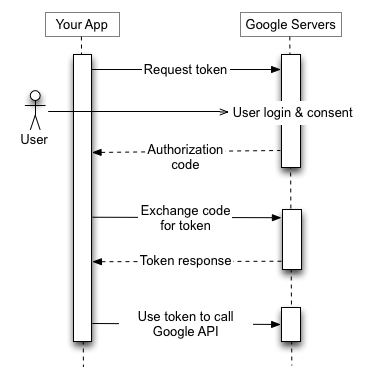
\includegraphics[scale=1]{Gambar/skenario1.png}
\caption[Skenario Aplikasi Layanan {\it Web}]{Skenario Aplikasi Layanan {\it
Web}}
\label{fig:skenarioaplikasiwebserver}
\end{figure}

\item Skenario Aplikasi yang Terinstal\\
Google OAuth 2.0 mendukung aplikasi yang diinstal pada perangkat seperti komputer, perangkat {\it mobile}, dan tablet. Ketika membuat klien id melalui Google Developers Console, menentukan aplikasi yang terinstal kemudian pilih Android, Chrome, iOS, atau "{\it Other}" sebagai jenis aplikasi. Hasil proses klien id dan kerahasiaan klien dalam beberapa kasus dimasukkan dalam kode sumber aplikasi. (Dalam konteks ini, kerahasiaan klien jelas tidak diperlakukan sebagai rahasia.)

Urutan otorisasi dimulai ketika aplikasi mengarahkan mesin pencari ke URL Google; URL termasuk parameter permintaan yang menunjukkan jenis akses yang diminta. Google menangani autentikasi pengguna, pemilihan sesi, dan izin pengguna. Hasilnya adalah sebuah kode otorisasi yang dapat ditukar untuk mendapatkan token akses dan memperbaharui token. Aplikasi harus menyimpan token yang diperbaharui untuk penggunaan masa depan dan menggunakan token akses untuk mengakses API Google. Setelah masa token akses berakhir, maka aplikasi akan memperbaharui token untuk mendapatkan yang baru. Untuk gambar skenario dapat dilihat pada Gambar \ref{fig:skenarioaplikasiyangterinstal}.

\begin{figure}[p]
\centering
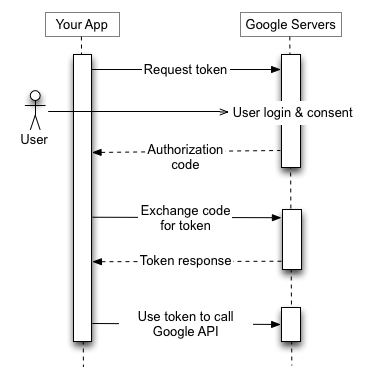
\includegraphics[scale=1]{Gambar/skenario1.png}
\caption[Skenario Aplikasi yang Terinstal]{Skenario Aplikasi yang Terinstal} 
\label{fig:skenarioaplikasiyangterinstal}
\end{figure}

\item Skenario Aplikasi Sisi Klien (JavaScript)\\
Google OAuth 2.0 mendukung aplikasi JavaScript yang berjalan di mesin pencari. Urutan otorisasi dimulai ketika aplikasi mengarahkan mesin pencari ke URL Google; URL termasuk parameter permintaan yang menunjukkan jenis akses yang diminta. Google menangani autentikasi pengguna, pemilihan sesi, dan izin pengguna. Hasilnya adalah token akses dimana klien harus melakukan validasi sebelum memasukkannya ke dalam permintaan Google API. Ketika masa token berakhir, aplikasi mengulangi proses. Untuk gambar skenario dapat dilihat pada Gambar \ref{fig:skenarioaplikasisisiklien}.

\begin{figure}[p]
\centering
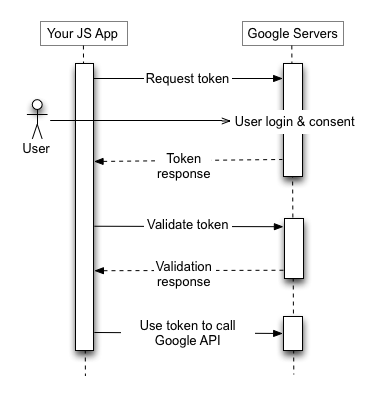
\includegraphics[scale=1]{Gambar/skenario2.png}
\caption[Skenario Aplikasi Sisi Klien (JavaScript)]{Skenario Aplikasi
Sisi Klien (JavaScript)}
\label{fig:skenarioaplikasisisiklien}
\end{figure}

\item Skenario Aplikasi Pada Perangkat Dengan Masukan Yang Terbatas\\
Google OAuth 2.0 mendukung aplikasi yang berjalan pada perangkat dengan masukan yang terbatas seperti konsol permainan, kamera video, dan printer. Urutan otorisasi dimulai dengan aplikasi membuat permintaan layanan {\it web} ke URL Google untuk kode otorisasi. Tanggapan berisi beberapa parameter, termasuk URL dan kode bahwa aplikasi menunjukkan kepada pengguna. Pengguna memperoleh URL dan kode dari perangkat, kemudian beralih ke perangkat terpisah atau komputer dengan kemampuan masukan yang lebih. Pengguna membuka mesin pencari, mengarahkan ke URL tertentu, melakukan {\it log in}, dan memasukan kode.

Sementara itu, aplikasi jajak pendapat dari URL Google pada interval tertentu. Setelah pengguna menyetujui akses, respon dari server Google berisi token akses dan memperbaharui token. Aplikasi harus menyimpan token yang baru untuk penggunaan masa depan dan menggunakan token akses untuk mengakses Google API. Setelah masa token akses berakhir, maka aplikasi akan memperbaharui token untuk mendapatkan yang baru. Untuk gambar skenario dapat dilihat pada Gambar \ref{fig:skenarioaplikasimasukanterbatas}.

\begin{figure}[p]
\centering
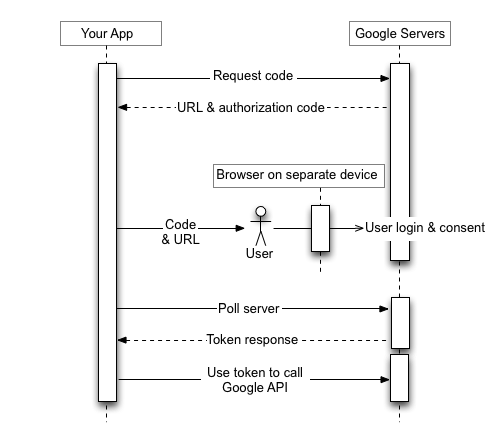
\includegraphics[scale=1]{Gambar/skenario3.png}
\caption[Skenario Aplikasi Pada Perangkat Dengan Masukan Yang
Terbatas]{Skenario Aplikasi Pada Perangkat Dengan Masukan Yang Terbatas}
\label{fig:skenarioaplikasimasukanterbatas}
\end{figure}

\item Skenario Layanan Akun\\
Google API seperti Prediction API dan Google Cloud Storage dapat bertindak atas nama aplikasi yang dibuat tanpa mengakses informasi pengguna. Dalam situasi ini aplikasi perlu membuktikan identitasnya sendiri ke API, tapi tidak diperlukan izin dari pihak pengguna. Demikian pula, dalam skenario perusahaan, aplikasi dapat meminta akses yang didelegasikan ke beberapa sumber daya.

Untuk jenis interaksi antara server memerlukan layanan akun, dimana akun tersebut terdapat pada aplikasi yang dibuat, bukan individu ke pengguna akhir. Aplikasi memanggil Google API atas nama layanan akun, dan izin dari pihak pengguna tidak diperlukan. (Dalam skenario tanpa layanan akun, aplikasi memanggil Google API atas nama pengguna akhir, dan izin dari pihak pengguna kadang-kadang diperlukan.)

Catatan: skenario layanan akun ini membutuhkan aplikasi untuk membuat dan tanda kriptografi JSON {\it Web Token} (JWTs). Sangat disarankan untuk menggunakan perpustakaan untuk melakukan tugas-tugas ini. Jika menulis kode untuk tanda penciptaan dan penandatanganan secara abstrak tanpa menggunakan perpustakaan, mungkin akan membuat kesalahan yang memiliki dampak yang parah pada keamanan aplikasi yang dibangun.

Mandat untuk layanan akun, yang diperoleh dari Google Developers Console, termasuk alamat email yang dihasilkan yang unik, klien id, dan setidaknya satu pasang kunci publik / privat. Menggunakan klien id dan satu kunci privat untuk membuat JWT (JSON {\it Web Token}) ditandatangani dan membangun permintaan token akses dalam format yang sesuai. Aplikasi kemudian mengirimkan permintaan token ke Google OAuth 2.0 Authorization Server, yang mengembalikan token akses. Aplikasi menggunakan token untuk mengakses API Google. Ketika masa token berakhir, aplikasi mengulangi proses. Untuk gambar skenario dapat dilihat pada Gambar \ref{fig:skenariolayananakun}.

\begin{figure}[h]
\centering
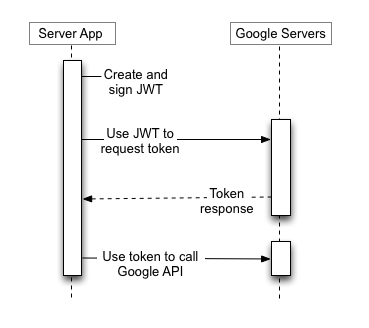
\includegraphics[scale=1]{Gambar/skenario4.png}
\caption[Skenario Layanan Akun]{Skenario Layanan Akun}
\label{fig:skenariolayananakun}
\end{figure}
\end{itemize}

\subsection{Masa Berlaku Token}
Kode token harus ditulis untuk mengantisipasi kemungkinan bahwa token yang diberikan mungkin tidak lagi bekerja suatu saat. Token mungkin berhenti bekerja untuk beberapa alasan di bawah ini:

\begin{itemize}
\item
Pengguna telah mencabut akses.
\item
Token tidak digunakan selama enam bulan.
\item
Akun pengguna telah melampaui jumlah tertentu permintaan token.
\end{itemize}

Saat ini batas untuk setiap akun Google adalah 25 token. Jika pengguna akun telah memiliki 25 token, permintaan autentikasi untuk token ke-26 akan berhasil tapi token yang paling tua atau token ke-1 akan dibuat tidak berlaku tanpa sepengetahuan pengguna. Jika perlu untuk melakukan otorisasi beberapa program, mesin, atau perangkat, salah satu solusi yang ditawarkan pihak Google adalah dengan membatasi jumlah klien, dimana satu pengguna harus melakukan otorisasi antara 15 hingga 20 akun. Jika anda adalah admin Google Apps, anda dapat membuat admin tambahan untuk mengizinkan beberapa klien.

\subsection{Lingkup Otorisasi \cite{Scope:2013}}
Lingkup disini merupakan sebuah {\it string} yang memungkinkan akses ke sumber daya tertentu, misalnya akses ke data pengguna. Dengan memasukan lingkup tertentu pada saat permintaan otorisasi, kemudian mendapatkan izin sesuai dengan teks yang akan ditampilkan ke pengguna. Setelah mendapat persetujuan dari pihak pengguna untuk izin atas lingkup tersebut, maka Google mengirimkan token untuk aplikasi yang mengidentifikasi untuk memberikan otorisasi khusus. Dengan kata lain, lingkup dan token menentukan apa saja data pengguna yang diberi izin oleh pengguna untuk diakses.

Sebuah aplikasi yang dibuat tanpa permintaan autentikasi (tidak ada lingkup yang diminta) hanya dapat mengakses data pengguna yang umum di Google+. Contoh, jika sebuah aplikasi mencari postingan publik, respon dari pencarian akan menampilkan id pengguna yang telah diposting secara publik dan aplikasi dapat mengakses nama dan URL foto pengguna yang dimana keduanya selalu diposting secara publik. Dapat juga mengakses tanggal ulang tahun atau jenis kelamin pengguna jika pengguna telah mempostinng secara publik. Untuk daftar lingkup otorisasi dapat dilihat pada daftar di bawah ini.

\begin{itemize}
\item Lingkup Profil\\
\begin{lstlisting}[basicstyle=\footnotesize]
profile
\end{lstlisting}
Lingkup ini merupakan lingkup dasar dimana lingkup ini melakukan beberapa hal sebagai berikut:
\begin{itemize}
\item
Meminta agar aplikasi diberikan akses ke informasi profil dasar bagi pengguna yang terautentikasi.
\item
Memungkinkan aplikasi untuk mengetahui siapa pengguna yang dikonfimasi dengan mengganti id pengguna dengan "{\it me}" yang mewakilkan pengguna yang telah terautentikasi disetiap permintaan yang dilakukan.
\item
Memungkinkan aplikasi diakses melalui aplikasi android.
\end{itemize}
\begin{lstlisting}[basicstyle=\footnotesize]
https://www.googleapis.com/auth/plus.login
\end{lstlisting}
Lingkup login disarankan untuk aplikasi yang menyediakan akses ke fitur sosial. Lingkup ini secara implisit mencakup lingkup profil dan juga meminta aplikasi
diberikan akses ke:
\begin{itemize}
\item
Rentang usia pengguna yang telah terautentikasi.
\item
Daftar teman yang telah diberikan akses oleh pengguna.
\item
Metode untuk membaca, menulis dan menghapus kegiatan app ke Google atas nama pengguna.
\end{itemize}
Lingkup ini juga memungkinkan lintas platform dengan pendaftaran tunggal.

\item Lingkup Email\\
\begin{lstlisting}[basicstyle=\footnotesize]
email
\end{lstlisting}
Lingkup ini meminta agar aplikasi diberikan akses ke:
\begin{itemize}
\item
Alamat email Google dari pengguna. Mengakses alamat email dengan memanggil people.get yang akan mengeluarkan {\it array} email atau dengan memanggil
\begin{lstlisting}[basicstyle=\footnotesize]
people.getOpenIdConnect
\end{lstlisting}
yang akan mengeluarkan email dengan format OIDC (OpenID Connect).
\item
Nama domain Google Apps jika ada yang dimiliki pengguna. Nama domain
dikembalikan sebagai kepemilikan domain dari people.get atau properti hd dari getOpenIdConnect.
\item
Lingkup email ini setara dan menggantikan lingkup di bawah ini.
\begin{lstlisting}[basicstyle=\footnotesize]
https://www.googleapis.com/auth/userinfo.email
\end{lstlisting}
\end{itemize}
\begin{lstlisting}[basicstyle=\footnotesize]
https://www.googleapis.com/auth/plus.profile.emails.read
\end{lstlisting}
Lingkup ini meminta aplikasi agar diberikan akses ke:
\begin{itemize}
\item
Alamat email Google pengguna yang telah diverifikasi di profil Google+. Mengakses email dengan memanggil people.get dan mengembalikan hasil email dalam {\it array}.
\item
Nama domain yang telah didaftarkan di Google jika pengguna memiliki fitur tersebut.
\end{itemize}

\item Lingkup yang lain\\
\begin{lstlisting}[basicstyle=\footnotesize]
openid
\end{lstlisting}
Lingkup openid menginformasikan server otorisasi bahwa klien membuat permintaan OpenID Connect dan meminta akses ke id pengguna yang terautentikasi tersebut. Lingkup ini harus disertakan lingkup OpenId Connect.

Metode getOpenIdConnect mengembalikan profil pengguna dengan format OIDC mengikuti jalur permintaan HTTP:
\begin{lstlisting}[basicstyle=\footnotesize]
https://www.googleapis.com/plus/v1/people/me/openIdConnect
\end{lstlisting}

Untuk keperluan login menggunakan lingkup profil atau lingkup
\begin{lstlisting}[basicstyle=\footnotesize]
https://www.googleapis.com/auth/plus.login
\end{lstlisting}
karena lingkup
\begin{lstlisting}[basicstyle=\footnotesize]
https://www.googleapis.com/auth/plus.me
\end{lstlisting}
tidak dianjurkan sebagai lingkup login dikarenakan pengguna yang belum {\it upgrade} ke Google+ tidak akan mengembalikan nama atau alamat email
pengguna.

Lingkup ini melakukan hal berikut:
\begin{itemize}
\item
Memungkinkan aplikasi untuk mengetahui siapa pengguna yang dikonfimasi dengan mengganti id pengguna dengan "{\it me}" yang mewakilkan pengguna yang telah terautentikasi disetiap permintaan yang dilakukan.
\end{itemize}

\item Lingkup yang tidak dipakai lagi\\
\begin{lstlisting}[basicstyle=\footnotesize]
https://www.googleapis.com/auth/userinfo.profile
\end{lstlisting}

Lingkup diatas sudah tidak dipakau lagi diganti dengan lingkup yang setara yaitu lingkup profil. Lingkup ini setara dengan lingkup profil dan meminta akses data yang sama. Catatan: lingkup ini tidak dipakai lagi namun tetap dipertahankan dan terus tersedia untuk kompatibilitas.

\begin{lstlisting}[basicstyle=\footnotesize]
https://www.googleapis.com/auth/userinfo.email
\end{lstlisting}

Lingkup diatas sudah tidak dipakau lagi diganti dengan lingkup yang setara yaitu lingkup email. Lingkup ini meminta akses ke alamat email akun Google pengguna. Google menghasilkan token baru dengan lingkup ini untuk titik akhir people.get. Lingkup ini juga meminta akses dari pengguna ke titik akhir userinfo unutk kompatibilitas.

Lihat juga lingkup terkait:
\begin{lstlisting}[basicstyle=\footnotesize]
https://www.googleapis.com/auth/plus.profile.emails.read
\end{lstlisting}
Catatan: lingkup ini tidak dipakai lagi namun tetap dipertahankan dan terus tersedia untuk kompatibilitas.
\end{itemize}

\subsection{API {\it Client Library} untuk PHP \cite{Lib:2015}}
Google OAuth menggunakan API {\it Client Library} untuk diimplemetasikan ke dalam bahasa pemrograman PHP. Sebelum itu ada beberapa langkah yang perlu diselesaikan sebelum menggunakan {\it library} ini. Beberapa langkat tersebut dapat dilihat di bawah ini.

\begin{itemize}
\item Jika belum memiliki akun Google, maka harus melakukan pendaftaran terlebih dahulu.
\item Jika belum pernah membuat proyek Google API, maka buat proyek di Developer Console Google.
\item Melakukan instal {\it library}.
\end{itemize}

Diperlukan pemahaman dasar-dasar untuk autentikasi dan otorisasi yang ditangani oleh API. Semua panggilan API harus menggunakan izin akses. Banyak metode API yang membutuhkan izin akses, tetapi beberapa ada yang tidak membutuhkan izin akses. Beberapa metode API yang dapat digunakan untuk berbagai kondisi, tergantung pada akses yang digunakan merupakan akses sederhana atau akses yang memerlukan izin. Berikut dua metode untuk menentukan jenis akses.

\begin{itemize}
\item Akses sederhana API (kunci API)\\
Metode ini tidak dapat digunakan untuk mengakses data pribadi pengguna. Aplikasi harus mengautentikasi sendiri sebagai aplikasi milik Google Developer Console {\it project}. Metode ini diperlukan untuk mengukur penggunaan proyek untuk tujuan akuntansi.
Konsep penting untuk kunci API pada saat mengautentikasi aplikasi, gunakan kunci API untuk proyek Google Developer Console yang dimiliki. Setiap akses sederhana untuk memanggil aplikasi harus menyertakan kunci ini. Peringatan dalam menggunakan kunci API, jika seseorang memperoleh kunci yang anda miliki maka mereka bisa menggunakan untuk memakan kuota atau dikenakan tuduhan terhadap proyek anda.

\item Akses otorisasi API (OAuth 2.0)\\
Metode ini digunakan untuk mengakses data pribadi pengguna. Sebelum mengakses otorisasi API, pengguna yang memiliki akses ke data pribadi harus memberikan akses ke aplikasi yang digunakan. Oleh karena itu, aplikasi yang digunakan harus disahkan, pengguna harus memberikan akses untuk aplikasi tersebut. Semua ini dapat dicapai dengan OAuth 2.0 dan {\it library}.
Konsep penting untuk OAuth 2.0 sebagai berikut.
    \begin{itemize}
    \item Ruang lingkup\\
    Setiap API mendefinisikan satu atau lebih lingkup yang menyatakan seperangkat operasi diizinkan. Sebagai contoh, sebuah API mungkin telah membaca saja atau mungkin telah membaca dan menulis lingkup. Ketika aplikasi meminta akses ke data pengguna, permintaan harus menyertakan satu atau lebih ruang lingkup. Pengguna perlu untuk menyetujui akses ruang lingkup yang diminta aplikasi anda.
    
    \item Pembaruan dan akses token\\
    Bila pengguna memberikan akses pada aplikasi, server otorisasi OAuth 2.0 menyediakan aplikasi dengan pembaruan dan akses token. Token ini hanya berlaku untuk ruang lingkup yang diminta. Aplikasi yang menggunakan token akses untuk mengotorisasi panggilan API. Token akses berakhir, tapi pembaruan token tidak. Aplikasi dapat menggunakan pembaruan token untuk mendapatkan token akses baru.
    Peringatan untuk menjauhkan pembaruan dan token akses pribadi. Jika seseorang memperoleh token anda, mereka bisa menggunakannya untuk mengakses data pribadi pengguna.
    
    \item ID klien dan rahasia klien\\
    ID klien dan rahasia klien merupakan sebuah {\it string} unik yang mengidentifikasi aplikasi yang digunakan dan digunakan untuk memperoleh token. Keduanya diciptakan untuk proyek Google Developers Console pada panel API Access yang terdapat pada Developer Console Google. Ada tiga jenis ID klien, jadi pastikan jenis yang digunakan sesuai dengan aplikasi yang akan digunakan. Berikut ketiga  jenis aplikasi.
    \begin{itemize}
    \item Web application client IDs
    \item Installed application client IDs
    \item Service Account client IDs
    \end{itemize}
    Peringatan untuk menjauhkan rehasia klien anda pribadi. Jika seseorang memperoleh rahasia klien anda, mereka bisa menggunakannya untuk mengkonsumsi kuota, dikenakan tuduhan terhadap proyek Google Developer Console, dan meminta akses ke data pengguna.
    \end{itemize}
\end{itemize}

Pada bagian terakhir ini menggambarkan bagaimana membangun suatu objek layanan API yang spesifik, membuat panggilan ke layanan, dan proses respon. Terdapat empat bagian untuk membangun dan memanggil layanan.

\begin{itemize}
\item Membangun objek klien \\
Objek klien adalah wadah utama untuk kelas dan konfigurasi di {\it library}.
\begin{lstlisting}[basicstyle=\footnotesize]
$client = new Google_Client();
$client->setApplicationName("My Application");
$client->setDeveloperKey("MY_SIMPLE_API_KEY");
\end{lstlisting}

\item Membangun layanan objek\\
Layanan dipanggil melalui permintaan untuk membangun layanan objek tertentu. Ini diciptakan dengan membangun layanan objek, dan melewati sebuah contoh dari \verb+Google_Client+ untuk itu. \verb+Google_Client+ berisi IO, autentikasi dan kelas-kelas lain yang diperlukan oleh layanan berfungsi, dan layanan menginformasikan klien yang menggunakan ruang lingkup untuk memberikan default ketika autentikasi pengguna.
\begin{lstlisting}[basicstyle=\footnotesize]
$service = new Google_Service_Books($client);
\end{lstlisting}

\item Memanggil API\\
Setiap API menyediakan sumber dan metode, biasanya terdapat di dalam rantai. Hal tersebut dapat diakses dari objek layanan dalam bentuk {\textdollar}service->resource->method(args). Kebanyakan metode memerlukan beberapa argumen, maka menerima parameter akhir dari {\it array} yang berisi parameter opsional. Misalnya, dengan Google Books API, kita dapat membuat panggilan ke daftar volume pencocokan {\it string} tertentu, dan menambahkan parameter filter yang opsional.
\begin{lstlisting}[basicstyle=\footnotesize]
$optParams = array('filter' => 'free-ebooks');
$results = $service->volumes->listVolumes('Henry David Thoreau', $optParams);
\end{lstlisting}

\item Penanganan hasil\\
Terdapat dua jenis respon utama yaitu item dan koleksi item. Masing-masing dapat diakses baik sebagai objek atau sebagai {\it array}. Koleksi penerapan antarmuka iterator sehingga dapat digunakan dalam konstruksi itu sendiri dan konstruksi lainnya.
\begin{lstlisting}[basicstyle=\footnotesize]
foreach ($results as $item) {
  echo $item['volumeInfo']['title'], "<br /> \n";
}
\end{lstlisting}
\end{itemize}

\section{Markdown}
\label{sec:markdown}

\subsection{Apa itu Markdown? \cite{Markguide:2015}}
John Gruber pembuat Markdown, memperkenalkan Markdown sebagai alat konfersi sebuah teks untuk ditampilkan ke HTML untuk para penulis {\it website}. Markdown memungkinkan penulis mudah untuk membaca dan mudah untuk menulis sebuah teks biasa, lalu merubah teks tersebut secara struktural yang valid dengan XHTML atau HTML. Markdown memiliki beberapa sintaks yang sederhana sebagai peraturan dalam menulis, hal tersebut membuat mudah dalam konfersi ke HTML dengan banyak perangkat lunak yang mendukung. Sebagai contoh, jika menulis \verb+**hello**+ pada Markdown dan konfersi ke HTML menggunakan teks editor yang mendukung, teks tersebut akan menjadi \verb+<strong>hello</hello>+ yang akan terlihat \textbf{hello}. 

\subsection{Sintaks yang Berguna \cite{Markguide:2015}}
Terdapat beberapa sintaks untuk penggunaan cetak tebal, cetak miring, judul sub bab, batas garis, paragraf, gambar, {\it link}, kode, kutipan, garis horisontal, dan daftar. Untuk penjelasan lebih lanjut dapat dilihat pada sub sub bab di bawah ini.

\begin{itemize}
\item Cetak Tebal dan Cetak Miring\\
Markdown memperlakukan karakter bintang (*) sebagai penekanan. Teks yang dibungkus dengan satu karakter * maka hasil teks akan cetak miring, dan teks yang dibungkus dengan dua karakter * maka hasil teks akan cetak tebal. Berikut contoh penggunaan sintaks untuk cetak tebal dan cetak miring.

\begin{lstlisting}[basicstyle=\footnotesize]
Alice melaporkan bahwa dirinya mengidap penyakit *Amyotrophic Lateral Sclerosis* sehingga mengganggu proses belajar.

Bob datang terlambat di kelas algoritma, dan **menolak untuk keluar** saat diusir dosen kelas.
\end{lstlisting}

Sintaks tersebut akan menghasilkan kode HTML sebagai berikut. Untuk hasil pada HTML dapat dilihat pada Gambar \ref{fig:cmct}.

\begin{lstlisting}[basicstyle=\footnotesize]
<p>Alice melaporkan bahwa dirinya mengidap penyakit <em>Amyotrophic Lateral Sclerosis</em> sehingga mengganggu proses belajar.</p>

<p>Bob datang terlambat di kelas algoritma, dan <strong>menolak untuk keluar</strong> saat diusir dosen kelas.</p>
\end{lstlisting}

\begin{figure}[H]
\centering
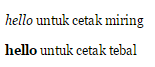
\includegraphics[scale=0.7]{Gambar/cmct.png}
\caption[Markdown Cetak Tebal dan Cetak Miring]{Markdown Cetak Tebal dan Cetak Miring}
\label{fig:cmct}
\end{figure}

\item Judul Bab\\
\item Markdown memperlakukan karakter hash (\#) sebagai indikator dari bab. Gunakan beberapa karakter hash untuk bab. Selalu gunakan spasi antara karakter hash dengan teks yang akan digunakan. Jumlah \# yang digunakan akan menentukan ukuran judul bab. Berikut contoh penggunaan sintaks untuk judul bab.
\begin{lstlisting}[basicstyle=\footnotesize]
# Bab 1
## Bab 1.1
### Bab 1.1.1
#### Bab 1.1.1.1
##### Bab 1.1.1.1.1
###### Bab 1.1.1.1.1.1
\end{lstlisting}
Sintaks tersebut akan menghasilkan kode HTML sebagai berikut. Untuk hasil pada HTML dapat dilihat pada Gambar \ref{fig:cmct}.
\begin{lstlisting}[basicstyle=\footnotesize]
<h1>Bab 1</h1>

<h2>Bab 1.1</h2>

<h3>Bab 1.1.1</h3>

<h4>Bab 1.1.1.1</h4>

<h5>Bab 1.1.1.1.1</h5>

<h6>Bab 1.1.1.1.1.1</h6>
\end{lstlisting}
\begin{figure}[H]
\centering
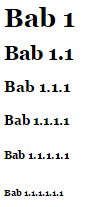
\includegraphics[scale=1]{Gambar/judulbab.png}
\caption[Markdown Judul Bab]{Markdown Judul Bab}
\label{fig:judulbab}
\end{figure}

\item Batas Baris\\
Untuk menyisipkan satu baris baru dalam dokumen, mengakhiri baris dengan dua spasi atau lebih lalu tekan '{\it Enter}'. Berikut contoh penggunaan sintaks untuk batas baris.
\begin{lstlisting}[basicstyle=\footnotesize]
Bob melihat pengumuman   
kelas PBO ditiadakan
\end{lstlisting}
Contoh di atas, setelah kata 'pengumuman' diakhiri dengan tiga spasi lalu tekan '{\it Enter}'. Sintaks tersebut akan menghasilkan kode HTML sebagai berikut. Untuk hasil pada HTML dapat dilihat pada Gambar \ref{fig:dengan}.
\begin{lstlisting}[basicstyle=\footnotesize]
<p>Bob melihat pengumuman <br />
kelas PBO ditiadakan</p>
\end{lstlisting}
\begin{figure}[H]
\centering
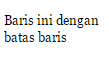
\includegraphics[scale=1]{Gambar/dengan.png}
\caption[Markdown Batas Baris Dengan Tiga Spasi]{Markdown Batas Baris
Dengan Tiga Spasi}
\label{fig:dengan}
\end{figure}
\begin{lstlisting}[basicstyle=\footnotesize]
Alice menunggu
kelas PBO
\end{lstlisting}
Contoh di atas, setelah kata 'menunggu' diakhiri tanpa spasi langsung tekan'Enter'. Sintaks tersebut akan menghasilkan kode HTML sebagai berikut. Untuk hasil pada HTML dapat dilihat pada Gambar \ref{fig:tanpa}.
\begin{lstlisting}[basicstyle=\footnotesize]
<p>Alice menunggu
kelas PBO</p>
\end{lstlisting}
\begin{figure}[H]
\centering
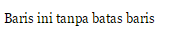
\includegraphics[scale=1]{Gambar/tanpa.png}
\caption[Markdown Batas Baris Tanpa Tiga Spasi]{Markdown Batas Baris
Tanpa Tiga Spasi}
\label{fig:tanpa}
\end{figure}

\item Paragraf\\
Untuk menyisipkan paragraf baru, cukup menyisipkan satu baris kosong. Berikut contoh penggunaan sintaks untuk paragraf.
\begin{lstlisting}[basicstyle=\footnotesize]
Alice memberikan tugas yang telah dititipkan Bob. Bob merasa Alice baik terhadap dirinya. Maka Bob mengirim pesan ke Alice.

Ternyata Alice mendapat hadiah dari tugas yang dititipkan oleh Bob.
\end{lstlisting}
Contoh diatas baris pertama adalah peragraf kesatu. Setelah itu ada satu baris kosong. Kalimat kedua merupakan paragraf kedua. Sintaks tersebut akan menghasilkan kode HTML sebagai berikut. Untuk hasil pada HTML dapat dilihat pada Gambar \ref{fig:tanpa}.
\begin{lstlisting}[basicstyle=\footnotesize]
<p>Alice memberikan tugas yang telah dititipkan Bob. Bob merasa Alice baik terhadap dirinya. Maka Bob mengirim pesan ke Alice.</p>

<p>Ternyata Alice mendapat hadiah dari tugas yang dititipkan oleh Bob.</p>
\end{lstlisting}
\begin{figure}[H]
\centering
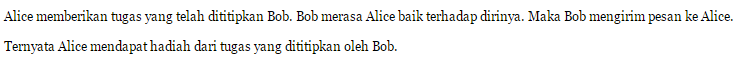
\includegraphics[scale=0.7]{Gambar/para.png}
\caption[Markdown Paragraf]{Markdown Paragraf}
\label{fig:para}
\end{figure}

\item Gambar\\
Untuk menyisipkan gambar pada dokumen Markdown, menggunakan sintaks berikut
\begin{lstlisting}[basicstyle=\footnotesize]
![teks](/url_gambar "judul_gambar")
\end{lstlisting}
Contoh penggunaan sintaks gambar: 
\begin{lstlisting}[basicstyle=\footnotesize]
![logo](https://www.google.com/logos/doodles/2014/googles-16th-birthday-4613606054297600-hp.gif "Google")
\end{lstlisting}
Url gambar dapat diganti dengan path yang mengarah pada {\it file} gambar yang akan digunakan. Sintaks tersebut akan menghasilkan kode HTML sebagai berikut. Untuk hasil pada HTML dapat dilihat pada Gambar \ref{fig:gambar}.
\begin{lstlisting}[basicstyle=\footnotesize]
<p><img src="https://www.google.com/logos/doodles/2014/googles-16th-birthday-4613606054297600-hp.gif" alt="logo" title="Google" /></p>
\end{lstlisting}
\begin{figure}[H]
\centering

\includegraphics[scale=1]{Gambar/gambar.png}
\caption[Markdown Menampilkan Gambar]{Markdown Menampilkan Gambar}
\label{fig:gambar}
\end{figure}

\item Link\\
Untuk menyisipkan {\it hyperlink} pada dokumen Markdown, gunakan sintaks berikut 
\begin{lstlisting}[basicstyle=\footnotesize]
[link_teks](/tujuan_url "judul opsional")
\end{lstlisting}
Contoh penggunaan sintaks link:
\begin{lstlisting}[basicstyle=\footnotesize]
[my_website](http://{\it browser}native.com "Click Here")
\end{lstlisting}
Sintaks tersebut akan menghasilkan kode HTML sebagai berikut. Untuk
hasil pada HTML dapat dilihat pada Gambar \ref{fig:ml}.
\begin{lstlisting}[basicstyle=\footnotesize]
<p><a href="http://{\it browser}native.com" title="Click Here">my_website</a></p>
\end{lstlisting}
\begin{figure}[H]
\centering
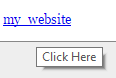
\includegraphics[scale=1]{Gambar/ml.png}
\caption[Markdown Link]{Markdown Link}
\label{fig:ml}
\end{figure}

\item Kode\\
Untuk menyisipkan kode pada sebuah baris pada dokumen Markdown, gunakan karakter
kutip belakang ('). Lampirkan kode yang ingin disisipkan dalam karakter kutip
belakang. Untuk menyisipkan blok kode gunakan tiga kutip belakang ('''). Setiap
baris kode harus diawali dengan empat spasi.
\begin{lstlisting}[basicstyle=\footnotesize]
Bob mendefinisikan fungsi penjumlahan()

'''
    fungsi penjumlahan(){
        A + 1 = C;
        2 + B = D
    }
'''
Paragraf lain.
\end{lstlisting}
'initLabels()' akan menjadi kode pada satu baris kalimat. Sedangkan fungsi yang ada didalam ''' akan menjadi blok kode. Sintaks tersebut akan menghasilkan kode HTML sebagai berikut. Untuk hasil pada HTML dapat dilihat pada Gambar
\ref{fig:kode}.
\begin{lstlisting}[basicstyle=\footnotesize]
<p>Bob mendefinisikan fungsi penjumlahan()</p>

<p>'''
    fungsi penjumlahan(){
        A + 1 = C;
        2 + B = D
    }
'''</p>
\end{lstlisting}
\begin{figure}[H]
\centering
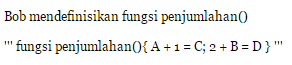
\includegraphics[scale=0.7]{Gambar/kode.png}
\caption[Markdown Kode]{Markdown Kode}
\label{fig:kode}
\end{figure}

\item Kutipan\\
Untuk menyisipkan kutipan pada dokumen Markdown, dapat menggunakan tanda lebih besar (>) pada awal kupitan.
\begin{lstlisting}[basicstyle=\footnotesize]
Alice mempunyai *quote* favorit:

> Kalau kamu mau, kamu pasti bisa
\end{lstlisting}
Sintaks tersebut akan menghasilkan kode HTML sebagai berikut. Untuk
hasil pada HTML dapat dilihat pada Gambar \ref{fig:kutipan}.
\begin{lstlisting}[basicstyle=\footnotesize]
<p>Alice mempunyai <em>quote</em> favorit:</p>

<blockquote>
  <p>Kalau kamu mau, kamu pasti bisa</p>
</blockquote>
\end{lstlisting}
\begin{figure}[H]
\centering
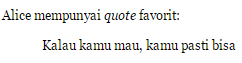
\includegraphics[scale=1]{Gambar/kutipan.png}
\caption[Markdown Kutipan]{Markdown Kutipan}
\label{fig:kutipan}
\end{figure}

\item Garis Horisontal\\
Menyisipkan garis horisontal pada dokumen Markdown, gunakan tiga atau lebih tanda hubung (-) dalam baris baru. Maka akan muncul sebagai garis horisontal pada keluaran HTML.
\begin{lstlisting}[basicstyle=\footnotesize]
# Pertemuan pertama kelas ASD

Bob dapat mengerti materi **Tree** dan **Hash** dengan cepat

---

Dirubah pada tanggal *13 Januari 2015*
\end{lstlisting}
Pada contoh di atas --- akan menjadi garis horisontal. Sintaks tersebut akan
menghasilkan kode HTML sebagai berikut. Untuk hasil pada HTML dapat dilihat pada
Gambar \ref{fig:garis}.
\begin{lstlisting}[basicstyle=\footnotesize]
<h1>Pertemuan pertama kelas ASD</h1>

<p>Bob dapat mengerti materi <strong>Tree</strong> dan <strong>Hash</strong> dengan cepat</p>

<hr />

<p>Dirubah pada tanggal <em>13 Januari 2015</em></p>

\end{lstlisting}
\begin{figure}[H]
\centering
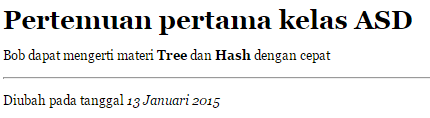
\includegraphics[scale=1]{Gambar/garis.png}
\caption[Markdown Garis Horisontal]{Markdown Garis Horisontal}
\label{fig:garis}
\end{figure}

\item Daftar\\
Terdapat dua macam daftar yang dapat dibuat. Dua macam daftar tersebut dapat dilihat dibawah ini.

\begin{enumerate}[(1)]
\item Daftar tidak berurutan\\
Untuk membuat daftar tidak berurutan dapat menggunakan simbol bintang *, simbol tambah +, maupun tanda hubung - sebelum daftar item yang ingin dimasukkan. Untuk contoh penggunaan dapat dilihat di bawah ini.
\begin{lstlisting}[basicstyle=\footnotesize]
* 13 Januari, Bob terlambat masuk kelas PBW
* 14 Januari, Bob terlambat masuk kelas PBO
* 15 Januari, Bob terlambat masuk kelas IMK

+ 16 Januari, Bob terlambat masuk kelas PBD
+ 17 Januari, Bob terlambat masuk kelas ASD
+ 18 Januari, Bob terlambat masuk kelas PBW ke 2

- 19 Januari, Bob terlambat masuk kelas IMK ke 2
- 20 Januari, Bob terlambat masuk kelas ASD ke 2
- 21 Januari, Bob terlambat masuk kelas PBO ke 2
\end{lstlisting}
Sintaks tersebut akan menghasilkan kode HTML sebagai berikut. Untuk
hasil pada HTML dapat dilihat pada Gambar \ref{fig:daftartidakberurutan}.
\begin{lstlisting}[basicstyle=\footnotesize]
<ul>
<li>13 Januari, Bob terlambat masuk kelas PBW</li>
<li>14 Januari, Bob terlambat masuk kelas PBO</li>
<li><p>15 Januari, Bob terlambat masuk kelas IMK</p></li>
<li><p>16 Januari, Bob terlambat masuk kelas PBD</p></li>
<li>17 Januari, Bob terlambat masuk kelas ASD</li>
<li><p>18 Januari, Bob terlambat masuk kelas PBW ke 2</p></li>
<li><p>19 Januari, Bob terlambat masuk kelas IMK ke 2</p></li>
<li>20 Januari, Bob terlambat masuk kelas ASD ke 2</li>
<li>21 Januari, Bob terlambat masuk kelas PBO ke 2</li>
</ul>
\end{lstlisting}
\begin{figure}[H]
\centering
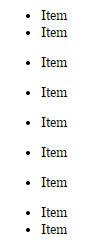
\includegraphics[scale=1]{Gambar/daftartidakberurutan.png}
\caption[Markdown Daftar Tidak Berurutan]{Daftar Tidak Berurutan}
\label{fig:daftartidakberurutan}
\end{figure}
\item Daftar berurutan\\
Untuk membuat daftar berurutan dapat menggunakan nomor sebelum daftar item yang
ingin dimasukkan. Untuk contoh penggunaan dapat dilihat di bawah ini.
\begin{lstlisting}[basicstyle=\footnotesize]
1. Bob aktif di dalam kelas PBWL 
2. Alice datang terlambat pada kelas PBWL
3. Carol mendapat nilai tertinggi untuk tugas akhir PBWL
\end{lstlisting}
Sintaks tersebut akan menghasilkan kode HTML sebagai berikut. Untuk
hasil pada HTML dapat dilihat pada Gambar \ref{fig:dafarberurutan}.
\begin{lstlisting}[basicstyle=\footnotesize]
<ol>
<li>Bob aktif di dalam kelas PBWL </li>
<li>Alice datang terlambat pada kelas PBWL</li>
<li>Carol mendapat nilai tertinggi untuk tugas akhir PBWL</li>
</ol>
\end{lstlisting}
\begin{figure}[H]
\centering
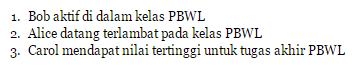
\includegraphics[scale=1]{Gambar/daftarberurutan.png}
\caption[Markdown Daftar Berurutan]{Markdown Daftar Berurutan}
\label{fig:dafarberurutan}
\end{figure}
\end{enumerate}
\end{itemize}

\subsection{GitHub Flavored Markdown \cite{Markdown:2015}}
GitHub menggunakan "GitHub Flavored Markdown" atau disingkat menjadi GFM. GFM berbeda dengan Standar Markdwon (SM) dalam beberapa bagian yang cukup signifikan dan ada beberapa sintaks tambahan. Beberapa hal yang berbeda dari SM dapat dilihat di bawah ini.

\begin{itemize}
\item Beberapa Garis Bawah Pada Kalimat\\
Pada Markdown kata yang berada dianatara garis bawah akan dirubah menjadi cetak miring, namun pada GFM garis bawah tidak memiliki pasangan maka garis bawah tersebut diabaikan sehingga akan tetap tampil sebagai karakter garis bawah.
\begin{lstlisting}[basicstyle=\footnotesize]
Bob_mempunyai_perangkat_canggih
terlihat_dari_apa_yang_dia_gunakan.
\end{lstlisting}
Hal tersebut memungkinkan untuk merender kode dan nama dengan benar. Untuk menekankan sebagian kata dapat menggunakan tanda bintang (*). Untuk hasil pada HTML dapat dilihat pada Gambar \ref{fig:gb}.
\begin{figure}[H]
\centering
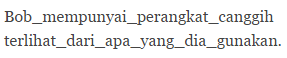
\includegraphics[scale=1]{Gambar/garisbawah.png}
\caption[GFM Garis Bawah]{GFM Garis Bawah}
\label{fig:gb}
\end{figure}

\item Taut Otomatis URL\\
GFM membuat standar untuk taut otomatis URL. Tanpa mengatur teks untuk link sebuah URL, cukup menyisipkan URL dan URL tersebut akan menjadi taut otomatis yang mengarah ke URL tersebut.
\begin{lstlisting}[basicstyle=\footnotesize]
http://www.unpar.ac.id
\end{lstlisting}
Link di atas kan menjadi taut secara otomatis ke URL tersebut. Untuk hasil pada HTML dapat dilihat pada Gambar \ref{fig:gfml}.
\begin{figure}[H]
\centering
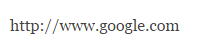
\includegraphics[scale=1]{Gambar/gfml.png}
\caption[GFM Taut Otomatis URL]{GFM Taut Otomatis URL}
\label{fig:gfml}
\end{figure}

\item Tanda Coret\\
GFM menambahkan sintaks untuk membuat teks dicoret, yang dihilangkan dari SM. Untuk membuat teks dicoret gunakan dua karakter tilde (~) antara kata yang akan dicoret.
\begin{lstlisting}[basicstyle=\footnotesize]
~~Dibuka kelas ASD pada masa SP.~~
\end{lstlisting}
Untuk hasil pada HTML dapat dilihat pada Gambar \ref{fig:tc}.
\begin{figure}[H]
\centering
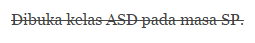
\includegraphics[scale=1]{Gambar/tc.png}
\caption[GFM Tanda Coret]{GFM Tanda Coret}
\label{fig:tc}
\end{figure}

\item Blok Kode\\
SM mengkonfersi blok kode dengan diawali empat spasi untuk setiap baris yang berada dalam blok kode. GFM juga mendukung blok kode namun cukup membungkus kode dengan tiga kutip belakang (''') tanpa harus memperhatikan empat spasi untuk awalan kode.
\begin{lstlisting}[basicstyle=\footnotesize]
Berikut kode **Java**

```
public class HelloWorld
{
	public static void main(String[] args) {
		System.out.println("Hello World!");
	}
}
```
\end{lstlisting}
Untuk hasil pada HTML dapat dilihat pada Gambar \ref{fig:blokkode}.
\begin{figure}[H]
\centering
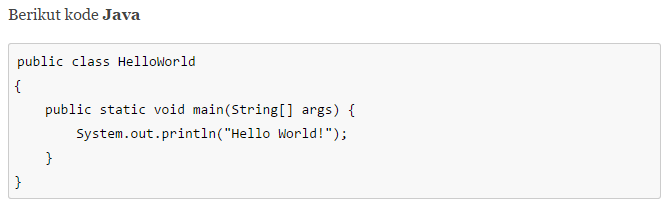
\includegraphics[scale=0.6]{Gambar/blokkode.png}
\caption[GFM Blok Kode]{GFM Blok Kode}
\label{fig:blokkode}
\end{figure}

\item Penandaan Sintaks\\
Blok kode dapat dilanjutkan dengan menambah sintaks. Dalam blok yang ditandai tambahkan sebuah indetifikasi bahasa apa yang digunakan. Misalnya penandaan kode untuk sintaks Java.
\begin{lstlisting}[basicstyle=\footnotesize]
```java
public class HelloWorld
{
	public static void main(String[] args) {
		System.out.println("Hello World!");
	}
}
```
\end{lstlisting}
Untuk hasil pada HTML dapat dilihat pada Gambar \ref{fig:ruby}.
\begin{figure}[H]
\centering
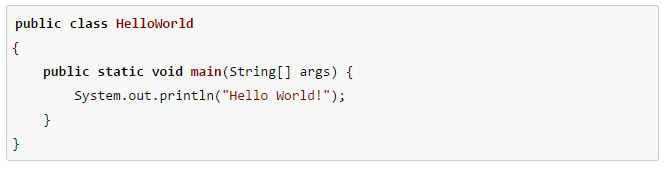
\includegraphics[scale=0.6]{Gambar/java.png}
\caption[GFM Penandaan Sintaks]{GFM Penandaan Sintaks}
\label{fig:ruby}
\end{figure}

\item Tabel\\
Dapat membuat tabel dengan menyusun daftar kata dan membagi dengan tanda hubung (-)untuk baris pertama. Kemudian memisahkan kolom dengan pipa |. Untuk contoh dapat diliahat di bawah ini.
\begin{lstlisting}[basicstyle=\footnotesize]
No  | Nama
--- | ---
1   | Bob
2   | Alice
\end{lstlisting}
Untuk hasil pada HTML dapat dilihat pada Gambar \ref{fig:t1}.
\begin{figure}[H]
\centering
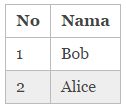
\includegraphics[scale=1]{Gambar/t1.png}
\caption[GFM Tabel 1]{GFM Tabel 1}
\label{fig:t1}
\end{figure}

Untuk tujuan estetika, dapat juga menambahkan pipa pada setiap ujung tabel. Untuk contoh dapat dilihat di bawah ini.
\begin{lstlisting}[basicstyle=\footnotesize]
| No  | Nama   |
| --- | ------ |
|  1  |  Bob   |
|  2  |  Alice |
\end{lstlisting}
Untuk hasil pada HTML dapat dilihat pada Gambar \ref{fig:t2}.
\begin{figure}[H]
\centering
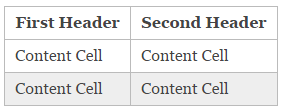
\includegraphics[scale=1]{Gambar/t2.png}
\caption[GFM Tabel 2]{GFM Tabel 2}
\label{fig:t2}
\end{figure}

Untuk membagi judul tabel dan isi tabel dapat menggunakan tanda hubung (-) yang tidak perlu disesuaikan dengan panjang judul tabel maupun isi tabel. Untuk contoh dapat dilihat di bawah ini.
\begin{lstlisting}[basicstyle=\footnotesize]
| Nama | Mata Kuliah yang Diambil  |
| ------------- | ----------- |
| Alice      | RPL|
| Bob     | PBWL     |
\end{lstlisting}
Untuk hasil pada HTML dapat dilihat pada Gambar \ref{fig:t3}.
\begin{figure}[H]
\centering
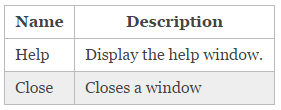
\includegraphics[scale=1]{Gambar/t3.png}
\caption[GFM Tabel 3]{GFM Tabel 3}
\label{fig:t3}
\end{figure}

Pada sintask tabel juga dapat memasukan berbagai sintaks Markdown kedalam tabel seperti link, cetak tebal, cetak miring atau teks yang dicoret. Untuk contoh dapat dilihat di bawah ini.
\begin{lstlisting}[basicstyle=\footnotesize]
| Nama | Deskripsi          |
| ------------- | ----------- |
| Alice      | ~~Terlambat~~ di setiap kelas.|
| Bob     | Seharusnya Bob _menjemput_ Alice     |
\end{lstlisting}
Untuk hasil pada HTML dapat dilihat pada Gambar \ref{fig:t4}.
\begin{figure}[H]
\centering
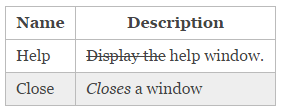
\includegraphics[scale=1]{Gambar/t4.png}
\caption[GFM Tabel 4]{GFM Tabel 4}
\label{fig:t4}
\end{figure}

Dengan memasukan tanda titik dua pada baris header. Dapat menentukan baris kiri,
baris tengah, maupun baris kanan. Untuk contoh dapat dilihat di bawah ini.
\begin{lstlisting}[basicstyle=\footnotesize]
| Rata Kiri  | Rata Tengah  | Rata Kanan |
| :--------- |:------------:| ----------:|
| Google     | Bob          | PBO        |
| Mozilla    | Carol        | PBW        |
| Opera      | Alice        | PBD        |
\end{lstlisting}
Untuk hasil pada HTML dapat dilihat pada Gambar \ref{fig:t5}.
\begin{figure}[H]
\centering
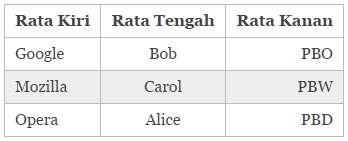
\includegraphics[scale=1]{Gambar/t5.png}
\caption[GFM Tabel 5]{GFM Tabel 5}
\label{fig:t5}
\end{figure}
\end{itemize}

\section{StrapdownJS \cite{Strapdownjs:2014}}
\label{sec:stapdownjs}

Strapdown.js merupakan sebuah teknologi untuk membuat dokumen Markdown menjadi lebih sederhana namun tetap elegan. Penggunaannya tidak diperlukan kompilasi dari sisi server. Gunakan strapdown.js untuk mendokumentasikan proyek dengan cepat, membuat tutorial, membuat halaman utama sebuah {\it website}. Contoh {\it website} yang menggunakan strapdown.js adalah http://strapdownjs.com/.

Untuk penggunaan StrapdownJS gunakan skrip strapdown.js dengan cara langsung mengarahkan ke {\it website} maupun menggunakan {\it path} yang mengarakan dimana {\it file} strapdown.js berada.
\begin{itemize}
\item Cara pertama:\\
\begin{lstlisting}[basicstyle=\footnotesize]
<script src="http://strapdownjs.com/v/0.2/strapdown.js"></script>
\end{lstlisting}
\item Cara kedua:\\
\begin{lstlisting}[basicstyle=\footnotesize]
<script src="v/0.2/strapdown.js"></script>
\end{lstlisting}
\end{itemize}

Peringatan untuk cara kedua harus terlebih dahulu mengunduh {\it file} strapdown.js.

Lalu buat {\it tag} <xml> untuk membuat area untuk menulis dengan sintaks Markdown.
\begin{lstlisting}[basicstyle=\footnotesize]
<xmp theme="united" style="display:none;">

</xmp>
\end{lstlisting}
Menulis dengan Markdown dapat dilakukan diantara  tag <xml> seperti di atas.

Untuk contoh lengkap penggunaan strapdown.js dapat dilihat pada template HTML
dibawah ini dan taruh pada {\it file} server statis untuk mencobanya:
\begin{lstlisting}[basicstyle=\footnotesize]
<!DOCTYPE html>
<html>
<title>Hello Strapdown</title>

<xmp theme="united" style="display:none;">
# Markdown text goes in here

## Chapter 1

Lorem ipsum dolor sit amet, consectetur adipisicing elit, sed do eiusmod tempor incididunt ut labore
et dolore magna aliqua. 

## Chapter 2

Ut enim ad minim veniam, quis nostrud exercitation ullamco laboris nisi ut
aliquip ex ea commodo consequat. Duis aute irure dolor in reprehenderit in voluptate velit esse
cillum dolore eu fugiat nulla pariatur. Excepteur sint occaecat cupidatat non proident, sunt in
culpa qui officia deserunt mollit anim id est laborum.
</xmp>

<script src="http://strapdownjs.com/v/0.2/strapdown.js"></script>
</html>
\end{lstlisting}

Strapdonw.js juga memiliki beberapa fitur :
\begin{enumerate}[(1)]
\item Ramah dengan mesin pencari
\item Kompatibel dengan berbagai {\it browser} (Sudah diuji dengan ponsel menggunakan
Safari, IE 8/9, Firefox, Chrome)
\item Github menggunakan Markdown (Tabel, Sintaks, Judul Bab)
\item Dapat menggunakan tema
\end{enumerate}

\section{Zurb Foundation \cite{Zurb:2015}}
\label{sec:zurbfoundation}

Zurb Foundation merupakan alat bantu dalam membuat aplikasi baru maupun membuat {\it website} yang responsif, tampilan antarmuka mengikuti lebar mesin pencari dan/atau layar komputer tanpa melakukan permintaan tambahan ke server. Jutaan desainer dan teknisi menggunakan Foundation sebagai bagian dari alur kerja mereka. Zurb Foundation adalah {\it framework} pertama yang memperkenalkan konsep responsif, semantik, mobile dan parsial. Zurb Foundation juga kompatibel dengan kebanyakan mesin pencari dan perangkat. Maka dari itu Zurb Foundation merupakan pilihan profesional bagi para desainer dan teknisi.

\subsection{Kompatibilitas}
Zurb Foundation dirancang dan diuji pada berbagai {\it browser} dan perangkat. Daftar pengujian pada berbagai {\it browser} dan perangkat dapat dilihat pada Tabel \ref{tab:kompatibilitas}.

%\newcommand{\Checkmark}{\ding{51}}%
%\newcommand{\XSolidBrush}{\ding{55}}%
\begin{table}
\centering
\caption[Tabel Daftar Pengujian Zurb Foundation]{Daftar Pengujian Zurb
Foundation\footnotemark[1]}
\label{tab:kompatibilitas}
\begin{tabular}{|l|l|l|l|}
\hline
{\it Browser}/OS & {\it The Grid} & {\it Layout}/UI & JS\\
\hline
Chrome & \Checkmark & \Checkmark & \Checkmark\\
\hline
Firefox & \Checkmark & \Checkmark & \Checkmark\\
\hline
Safari & \Checkmark & \Checkmark & \Checkmark\\
\hline
IE10 & \Checkmark & \Checkmark & \Checkmark\\
\hline
IE11 & \Checkmark & \Checkmark & \Checkmark\\
\hline
IE9 & \Checkmark & \Checkmark & \Checkmark\\
\hline
IE8 & \XSolidBrush & \XSolidBrush & \XSolidBrush\\
\hline
IE7 & \XSolidBrush & \XSolidBrush & \XSolidBrush\\
\hline
iOS (iPhone) & \Checkmark & \Checkmark & \Checkmark\\
\hline
iOS (iPad) & \Checkmark & \Checkmark & \Checkmark\\
\hline
Android 2, 4 (Phone) & \Checkmark & \Checkmark & \Checkmark\\
\hline
Android 2, 4 (Tablet) & \Checkmark & \Checkmark & \Checkmark\\
\hline
Windows Phone 7+ & \Checkmark & \Checkmark & \Checkmark\\
\hline
Surface & \Checkmark & \Checkmark & \Checkmark\\
\hline
\end{tabular}
\end{table}

\footnotetext[1]{http://foundation.zurb.com/docs/compatibility.html}

\subsection{Apa Saja yang Dapat Dibuat dengan Foundation?}
Foundation memiliki banyak komponen dan struktur untuk membantu membangun sebuah situs responsif. Untuk komponen Foundation dapat melihat beberapa gambar dibawah ini:

\begin{enumerate}[(1)]
\item {\it Grid}\\
{\it Grid} bekerja pada hampir semua perangkat dan memiliki dukungan untuk menjadi satu kesatuan, sumber pemesanan, {\it offset} dan perangkat presentasi. Hal tersebut sedikit mudah dengan waktu yang singkat dapat menciptakan tata letak yang kompleks seperti ini. Untuk contoh {\it grid} dapat dilihat pada Gambar \ref{fig:grid}.

\begin{figure}[H]
\centering
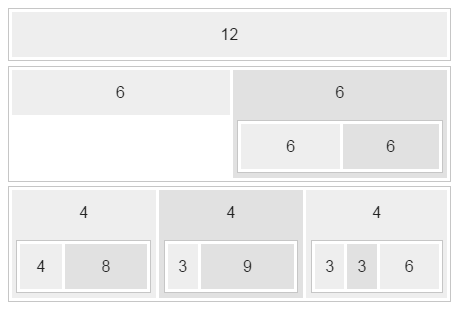
\includegraphics[scale=0.7]{Gambar/grid.png}
\caption[Contoh {\it Grid} Zurb Foundation]{Contoh {\it Grid} Zurb Foundation}
\label{fig:grid}
\end{figure}

\begin{itemize}
\item {\it Grid} Utama\\
Mulailah membuat elemen dengan kelas secara berturu-turut. Ini akan membuat blok horisontal yang berisi kolom vertikal. Kemudian tambahkan beberapa div dengan kelas kolom pada baris tersebut. Dapat menggunakan {\it column} atau {\it columns} karena hanya berbeda tata bahasa. Tentukan lebar dari setiap kolom dengan menggunakan kelas {\it small}-\#, {\it medium}-\#, dan {\it large}-\#. Foundation merupakan yang pertama dalam mengembangkan kode untuk layar kecil dan untuk perangkat dengan layar lebih besar akan mendapat bagian dengan gaya yang sama. Berikut kode HTML untuk membuat grid utama dan dapat dilihat hasilnya pada Gambar \ref{fig:gridutama}.
\begin{lstlisting}[basicstyle=\footnotesize]
<!-- no. 1 -->
<div class="row">
<div class="small-2 large-4 columns">2</div>
<div class="small-4 large-4 columns">4</div>
<div class="small-6 large-4 columns">6</div>
</div>
<!-- no. 2 -->
<div class="row">
<div class="large-3 columns">full</div>
<div class="large-6 columns">full</div>
<div class="large-3 columns">full</div>
</div>
<!-- no. 3 -->
<div class="row">
<div class="small-6 large-2 columns">6</div>
<div class="small-6 large-8 columns">6</div>
<div class="small-12 large-2 columns">full</div>
</div>
<!-- no. 4 -->
<div class="row">
<div class="small-3 columns">3</div>
<div class="small-9 columns">9</div>
</div>
<!-- no. 5 -->
<div class="row">
<div class="large-4 columns">full</div>
<div class="large-8 columns">full</div>
</div>
<!-- no. 6 -->
<div class="row">
<div class="small-6 large-5 columns">6</div>
<div class="small-6 large-7 columns">6</div>
</div>
<!-- no. 7 -->
<div class="row">
<div class="large-6 columns">full</div>
<div class="large-6 columns">full</div>
</div>
\end{lstlisting}
\begin{figure}[H]
\centering
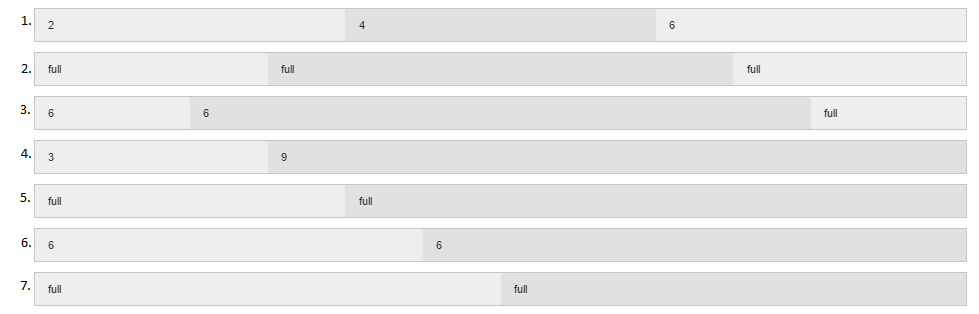
\includegraphics[scale=0.6]{Gambar/gridutama.png}
\caption[{\it Grid} Utama]{{\it Grid} Utama}
\label{fig:gridutama}
\end{figure}
\item {\it Grid} Kecil\\
Menampilkan {\it grid} kecil ke layar besar lebih mudah dibandingkan menampilkan {\it grid} besar ke layar kecil. Berikut kode HTML untuk membuat {\it grid} kecil dan dapat dilihat hasilnya pada Gambar \ref{fig:gridkecil}.
\begin{lstlisting}[basicstyle=\footnotesize]
<!-- no. 1 -->
<div class="row">
<div class="small-2 columns">2 columns</div>
<div class="small-10 columns">10 columns</div>
</div>
<!-- no. 2 -->
<div class="row">
<div class="small-3 columns">3 columns</div>
<div class="small-9 columns">9 columns</div>
</div>
\end{lstlisting}
\begin{figure}[H]
\centering
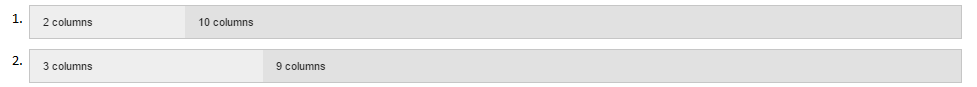
\includegraphics[scale=0.6]{Gambar/gridkecil.png}
\caption[{\it Grid} Kecil]{{\it Grid} Kecil}
\label{fig:gridkecil}
\end{figure}
\item {\it Grid} Menengah\\
Layar berukuran sedang akan mendapatkan bagian dari gaya yang kecil, kecuali ditentukan tata letak yang berbeda dengan menggunakan {\it grid} menengah. Berikut kode HTML untuk membuat {\it grid} menengah dan dapat dilihat hasilnya pada Gambar \ref{fig:gridmenengah}.
\begin{lstlisting}[basicstyle=\footnotesize]
<!-- no. 1 -->
<div class="row">
<div class="medium-2 columns">2 columns</div>
<div class="medium-10 columns">10 columns</div>
</div>
<!-- no. 2 -->
<div class="row">
<div class="medium-3 columns">3 columns</div>
<div class="medium-9 columns">9 columns</div>
</div>
\end{lstlisting}
\begin{figure}[H]
\centering
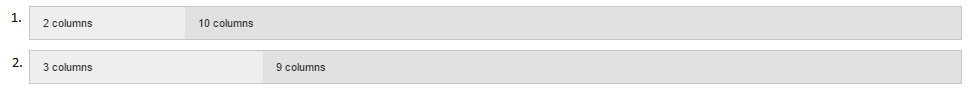
\includegraphics[scale=0.6]{Gambar/gridmenengah.png}
\caption[{\it Grid} Menengah]{{\it Grid} Menengah}
\label{fig:gridmenengah}
\end{figure}

\item {\it Grid} Tingkat Lanjut\\
Dapat membuat {\it grid} bersarang dengan menggunakan kode HTML berikut. Untuk hasilnya dapat dilihat pada Gambar \ref{fig:gridadv}.
\begin{lstlisting}[basicstyle=\footnotesize]
<div class="row">
<div class="small-8 columns">8
<div class="row">
<div class="small-8 columns">8 Nested
<div class="row">
<div class="small-8 columns">8 Nested Again</div>
<div class="small-4 columns">4</div>
</div>
</div>
<div class="small-4 columns">4</div>
</div>
</div>
<div class="small-4 columns">4</div>
</div>
\end{lstlisting}
\begin{figure}[H]
\centering
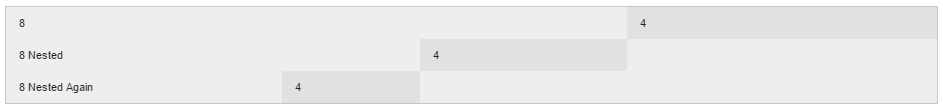
\includegraphics[scale=0.6]{Gambar/gridadv.png}
\caption[{\it Grid} Tingkat Lanjut]{{\it Grid} Tingkat Lanjut}
\label{fig:gridadv}
\end{figure}

\item {\it Grid} Dengan Offset\\
Memindahkan blok hingga 11 kolom ke kanan dengan menggunakan kelas
{\it large-offset}-1 dan {\it small-offset}-3. Berikut contoh penggunaan pada kode HTML dan dapat dilihat hasilnya pada Gambar \ref{fig:gridoffset}.
\begin{lstlisting}[basicstyle=\footnotesize]
<!-- no. 1 -->
<div class="row">
<div class="large-1 columns">1</div>
<div class="large-11 columns">11</div>
</div>
<!-- no. 2 -->
<div class="row">
<div class="large-1 columns">1</div>
<div class="large-10 large-offset-1 columns">10, offset 1</div>
</div>
<!-- no. 3 -->
<div class="row">
<div class="large-1 columns">1</div>
<div class="large-9 large-offset-2 columns">9, offset 2</div>
</div>
<!-- no. 4 -->
<div class="row">
<div class="large-1 columns">1</div>
<div class="large-8 large-offset-3 columns">8, offset 3</div>
</div>
\end{lstlisting}
\begin{figure}[H]
\centering
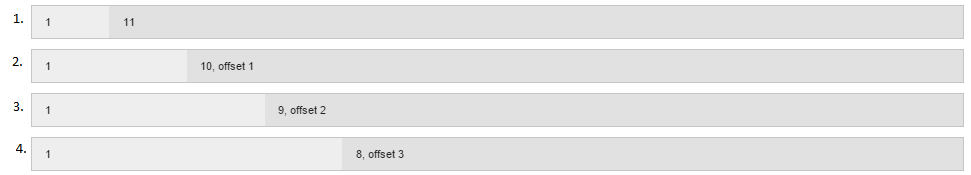
\includegraphics[scale=0.6]{Gambar/gridoffset.png}
\caption[{\it Grid} Dengan Offset]{{\it Grid} Dengan Offset}
\label{fig:gridoffset}
\end{figure}
\item {\it Grid} Dengan Baris yang Tidak Lengkap\\
Untuk mengatasi perbedaan pada beberapa mesin pencari, Foundation akan
memindahkan kolom terakhir berturut-turut ke kanan sehingga sejajar dengan tepi. Jika jumlah kolom tidak mencapai 12 maka pada kolom terakhir perlu ditandai dengan kelas {\it end}. Berikut contoh penggunaan pada kode HTML dan dapat dilihat hasilnya pada Gambar \ref{fig:gridtidaklengkap}.
\begin{lstlisting}[basicstyle=\footnotesize]
<!-- no. 1 -->
<div class="row">
<div class="medium-3 columns">3</div>
<div class="medium-3 columns">3</div>
<div class="medium-3 columns">3</div>
</div>
<!-- no. 2 -->
<div class="row">
<div class="medium-3 columns">3</div>
<div class="medium-3 columns">3</div>
<div class="medium-3 columns end">3 end</div>
</div>
\end{lstlisting}
\begin{figure}[H]
\centering
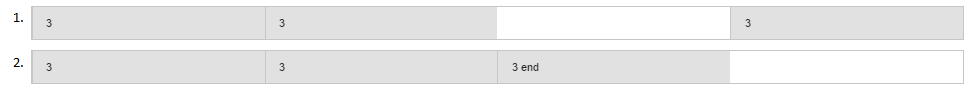
\includegraphics[scale=0.6]{Gambar/gridtidaklengkap.png}
\caption[{\it Grid} Dengan Baris yang Tidak Lengkap]{{\it Grid} Dengan Baris yang Tidak Lengkap}
\label{fig:gridtidaklengkap}
\end{figure}

item {\it Grid} Dengan Baris yang Mengempis/Tidak Mengempis\\
Kelas ini memungkinkan untuk menghapus jarak antara kolom. Ada kondisi dimana tidak setiap kueri memiliki sifat {\it collapsed} atau {\it uncollapsed}, cukup menambahkan kelas yang mengatur hal tersebut. Misal tidak menunjukkan jarak antara kolom pada kolom ukuran kecil dan menambahkan jarak antara komlom pada kolom ukuran menengah. Berikut contoh penggunaan pada kode HTML dan dapat dilihat hasilnya pada Gambar \ref{fig:gridmengempis}.
\begin{lstlisting}[basicstyle=\footnotesize]
<div class="row medium-uncollapse large-collapse">
<div class="small-6 columns">
Removes gutter at large media query
</div>
<div class="small-6 columns">
Removes gutter at large media query
</div>
</div>
\end{lstlisting}
\begin{figure}[H]
\centering
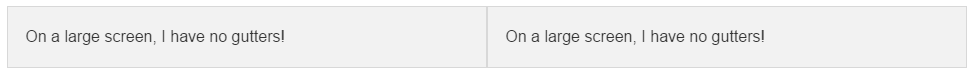
\includegraphics[scale=0.6]{Gambar/gridmengempis.png}
\caption[{\it Grid} Dengan Baris yang Mengempis/Tidak Mengempis]{{\it Grid} Dengan Baris yang Mengempis/Tidak Mengempis}
\label{fig:gridmengempis}
\end{figure}

\item {\it Grid} Dengan Kolom yang Berpusat\\
Dengan menambahkan kelas {\it small-centered} pada kolom tersebut dapat membuat kolom yang berpusat. Tampilan pada layar besar akan mendapat bagian seperti tampilan pada layar kecil, tapi dapat menggunakan kelas {\it large-centered} untuk memusatkan di tampilan pada layar besar. Untuk tidak memusatkan di tampilan pada layar besar dapat menggunakan {\it large-uncentered}. Berikut contoh penggunaan pada kode HTML dan dapat dilihat hasilnya pada Gambar \ref{fig:gridkolomberpusat}.
\begin{lstlisting}[basicstyle=\footnotesize]
<!-- no. 1 -->
<div class="row">
<div class="small-3 small-centered columns">3 centered</div>
</div>
<!-- no. 2 -->
<div class="row">
<div class="small-6 large-centered columns">6 centered</div>
</div>
<!-- no. 3 -->
<div class="row">
<div class="small-9 small-centered large-uncentered columns">9 centered</div>
</div>
<!-- no. 4 -->
<div class="row">
<div class="small-11 small-centered columns">11 centered</div>
</div>
\end{lstlisting}
\begin{figure}[H]
\centering
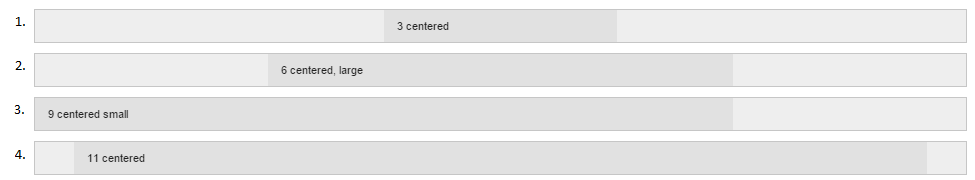
\includegraphics[scale=0.6]{Gambar/gridkolomberpusat.png}
\caption[{\it Grid} Dengan Kolom yang Berpusat]{{\it Grid} Dengan Kolom yang Berpusat}
\label{fig:gridkolomberpusat}
\end{figure}

\item {\it Grid} Dengan Sumber yang Terurut\\
Dengan menggunakan kelas {\it push} dan {\it pull} memungkinkan untuk memindahkan kolom sesuai dengan titik yang ditentukan. Jika memiliki sub menu di bawah menu utama pada layar kecil, maka memiliki pilihan untuk posisi sub navigasi di kanan atau di kiri untuk tampilan pada layar besar. Berikut contoh penggunaan pada kode HTML dan dapat dilihat hasilnya pada Gambar \ref{fig:gridsumberterurut}.
\begin{lstlisting}[basicstyle=\footnotesize]
<!-- no. 1 -->
<div class="row">
<div class="small-10 small-push-2 columns">10</div>
<div class="small-2 small-pull-10 columns">2, last</div>
</div>
<!-- no. 2 -->
<div class="row">
<div class="large-9 large-push-3 columns">9</div>
<div class="large-3 large-pull-9 columns">3, last</div>
</div>
<!-- no. 3 -->
<div class="row">
<div class="large-8 large-push-4 columns">8</div>
<div class="large-4 large-pull-8 columns">4, last</div>
</div>
<!-- no. 4 -->
<div class="row">
<div class="small-5 small-push-7 medium-7 medium-push-5 columns">7</div>
<div class="small-7 small-pull-5 medium-5 medium-pull-7 columns">5, last</div>
</div>
<!-- no. 5 -->
<div class="row">
<div class="medium-6 medium-push-6 columns">6</div>
<div class="medium-6 medium-pull-6 columns">6, last</div>
</div>
\end{lstlisting}
\begin{figure}[H]
\centering
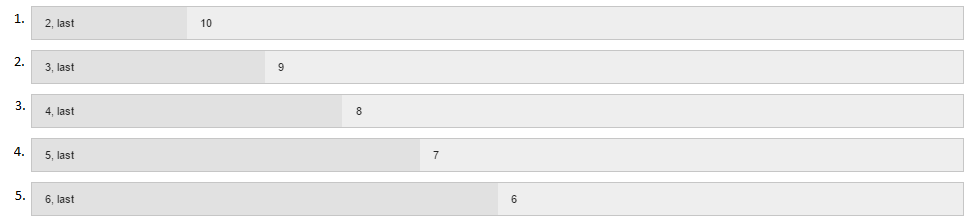
\includegraphics[scale=0.6]{Gambar/gridsumberterurut.png}
\caption[{\it Grid} Dengan Sumber yang Terurut]{{\it Grid} Dengan Sumber yang Terurut}
\label{fig:gridsumberterurut}
\end{figure}
\end{itemize}

\item Tombol\\
Mengklik tombol dengan material yang bagus merupakan hal yang mengagumkan. Mengklik tombol juga menghubungkan pengguna dengan berbagai aksi. Ada beberapa gaya tombol yang ringan untuk ukuran, presentasi, dan warna untuk menyesuaikan tombol Anda sendiri semudah menambahkan kelas. Untuk contoh macam-macam tombol dapat dilihat pada Gambar \ref{fig:button}.

\begin{figure}[H]
\centering
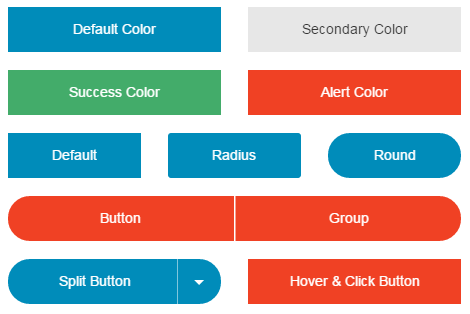
\includegraphics[scale=0.7]{Gambar/button.png}
\caption[Contoh Tombol Zurb Foundation]{Contoh Tombol Zurb Foundation}
\label{fig:button}
\end{figure}

\begin{itemize}
\item Tombol Utama\\
Dapat membuat tombol utama dengan kode HTML sebagai berikut dan dapat
dilihat hasilnya pada Gambar \ref{fig:tomboldasar}.
\begin{lstlisting}[basicstyle=\footnotesize]
<a href="#" class="button">Default Button</a>
\end{lstlisting}
\begin{figure}[H]
\centering
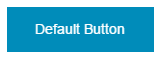
\includegraphics[scale=1]{Gambar/tomboldasar.png}
\caption[Tombol Dasar]{Tombol Dasar}
\label{fig:tomboldasar}
\end{figure}
\item Mengubah Ukuran Tombol\\
Terdapat kelas tambahan untuk merubah bentuk dan ukuran tombol, berikut kode HTML yang dapat digunakan dan dapat dilihat hasilnya pada Gambar \ref{fig:ukurantombol}.
\begin{lstlisting}[basicstyle=\footnotesize]
<!-- Kelas untuk merubah ukuran -->
1. <a href="#" class="button tiny">Tiny Button</a>
2. <a href="#" class="button small">Small Button</a>
3. <a href="#" class="button">Default Button</a>
4. <a href="#" class="button disabled">Disabled Button</a>
5. <a href="#" class="button large">Large Button</a>
6. <a href="#" class="button expand">Expanded Button</a>
<!-- Kelas untuk merubah bentuk -->
7. <a href="#" class="button round">Round Button</a>
8. <a href="#" class="button radius">Radius Button</a>
\end{lstlisting}
\begin{figure}[H]
\centering
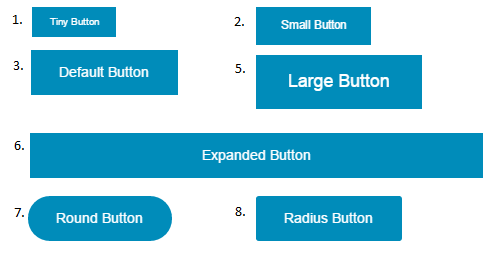
\includegraphics[scale=1]{Gambar/ukurantombol.png}
\caption[Ukuran dan Bentuk Tombol]{Ukuran dan Bentuk Tombol}
\label{fig:ukurantombol}
\end{figure}
\item Warna Tombol\\
Terdapat kelas tambahan untuk merubah warna tombol, berikut kode HTML yang dapat digunakan dan dapat dilihat hasilnya pada Gambar \ref{fig:warnatombol}.
\begin{lstlisting}[basicstyle=\footnotesize]
<!-- Kelas untuk merubah warna -->
1. <a href="#" class="button">Default Button</a>
2. <a href="#" class="button success">Success Button</a>
3. <a href="#" class="button secondary">Secondary Button</a>
4. <a href="#" class="button alert">Alert Button</a>
5. <a href="#" class="button info">Info Button</a>
6. <a href="#" class="button disabled">Disabled Button</a>
\end{lstlisting}
\begin{figure}[H]
\centering
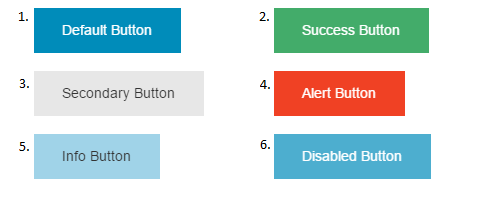
\includegraphics[scale=1]{Gambar/warnatombol.png}
\caption[Warna-warna Tombol]{Warna-warna Tombol}
\label{fig:warnatombol}
\end{figure}
\item Aksesbilitas\\
Gunakan kode HTML dibawah ini untuk membuat tombol lebih mudah diakses. Dapat menggunakan atribut aria-label='submit form' untuk memberikan petunjuk jika tidak ada keterangan pada tombol. Jika tombol tidak memiliki <a href=""> maka cukup menambahkan tabindex="0" pada div atau span untuk membuat tombol tersebut dapat difokuskan.
\begin{lstlisting}[basicstyle=\footnotesize]
1. <a role="button" href="#" class="button">Default Button</a>
2. <a role="button" aria-label="submit form" href="#" class="button">Submit</a>
3. <div role="button" tabindex="0" class="button">Default Button</div>
\end{lstlisting}
\begin{figure}[H]
\centering
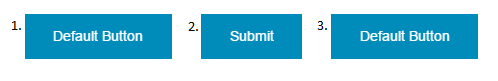
\includegraphics[scale=1]{Gambar/aksesbilitastombol.png}
\caption[Aksesbilitas Tombol]{Aksesbilitas Tombol}
\label{fig:aksesbilitastombol}
\end{figure}
\end{itemize}

\item Tabel\\
Dapat membuat tabel dengan menggunakan markup yang minim. Berikut contoh penggunaan tabel pada kode HTML dan dapat dilihat hasilnya pada Gambar \ref{fig:tabel}.
\begin{lstlisting}[basicstyle=\footnotesize]
<table>
  <thead>
    <tr>
      <th width="200">Table Header</th>
      <th>Table Header</th>
      <th width="150">Table Header</th>
      <th width="150">Table Header</th>
    </tr>
  </thead>
  <tbody>
    <tr>
      <td>Content Goes Here</td>
      <td>This is longer content Donec id elit non mi porta gravida at eget metus.</td>
      <td>Content Goes Here</td>
      <td>Content Goes Here</td>
    </tr>
    <tr>
      <td>Content Goes Here</td>
      <td>This is longer Content Goes Here Donec id elit non mi porta gravida at eget metus.</td>
      <td>Content Goes Here</td>
      <td>Content Goes Here</td>
    </tr>
    <tr>
      <td>Content Goes Here</td>
      <td>This is longer Content Goes Here Donec id elit non mi porta gravida at eget metus.</td>
      <td>Content Goes Here</td>
      <td>Content Goes Here</td>
    </tr>
  </tbody>
</table>
\end{lstlisting}
\begin{figure}[H]
\centering
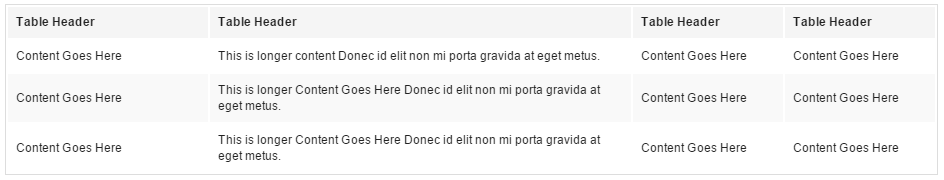
\includegraphics[scale=0.6]{Gambar/tabel.png}
\caption[Tabel Foundation]{Tabel Foundation}
\label{fig:tabel}
\end{figure}
\item Navigasi\\
Orang yang mengakses harus bisa berkeliling melihat menu-menu yang ada. Gaya navigasi pada Foundation meliputi : bar bagian atas yang kuat dengan menu dropdown; tombol; bar pencari; ikon bar yang keren; implementasi kanvas yang lepas dari keluhan; dan sekelompok navigasi lainnya. Untuk contoh macam-macam navigasi dapat dilihat pada Gambar \ref{fig:navi}.
\begin{figure}[ht]
\centering
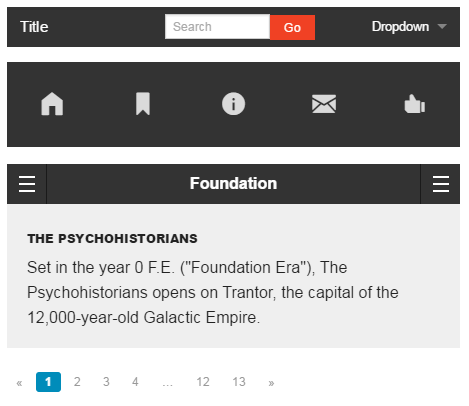
\includegraphics[scale=0.9]{Gambar/navigation.png}
\caption[Contoh Navigasi Zurb Foundation]{Contoh Navigasi Zurb Foundation}
\label{fig:navi}
\end{figure}

\item {\it Plugins}\\
Sudah meliputi banyak {\it plugin} JavaScript yang ditulis untuk modal dasar {\it pop-up}; menambat formulir validasi yang diperlukan; membuat {\it tab} konten; tanda peringatan; dan masih banyak lagi. Untuk contoh macam-macam {\it plugin} dapat dilihat pada Gambar \ref{fig:plugin}.

\begin{figure}[ht]
\centering
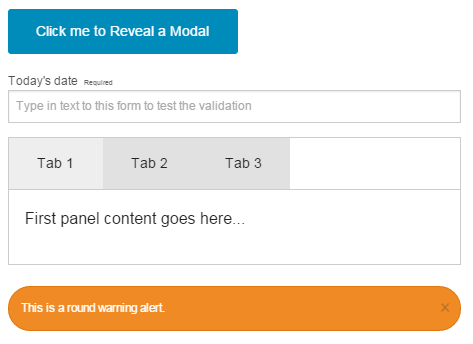
\includegraphics[scale=0.9]{Gambar/plugin.png}
\caption[Contoh Plugins Zurb Foundation]{Contoh Plugins Zurb Foundation}
\label{fig:plugin}
\end{figure}

\end{enumerate}